\chapter{Visualisation expérimental d'un mode localisé}
Comme vu précédemment, un défaut dans le réseau provoque un mode localisé. L'objectif est ici de mettre en évidence ce phénomène de manière expérimentale.\\


Un mode localisé dans un tel réseau est à la fois difficile à générer et à observer, expérimentalement comme numériquement. La fréquence de résonance du défaut doit se trouver sur le bord intérieur d'une bande interdite afin de pouvoir la visualiser sur les coefficients de transmission et réflexion. En effet, la propagation de l'onde dans le réseau se fait sur une longueur réduite : la bande interdite rend la décroissance de l'onde exponentielle. Par conséquent, la fréquence de résonance du défaut et la position du défaut par rapport à la source sont cruciales. De plus, une fois le mode généré, il ne peut être observé que très localement et si le réseau est trop grand, il n'est alors pas visible sur les coefficients de transmission et de réflexion qui sont issues de mesures à l'entrée et la sortie du réseau.


\section{Protocole expérimental}
Le banc de mesure utilisé est constitué d'un tuyau perforé de 60 trous sur lesquels peuvent être fixés soit des résonateurs de longueurs de cavité variables (les dimensions sont présentes en annexe), soit des bouchons (cf figure~\ref{photo_manip}). La source utilisée est celle du capteur d'impédance (piézoélectrique). Celui-ci est préalablement calibré, puis fixé à une des extrémités du réseau et est relié à une carte d'acquisition piloté par le logiciel spécialisé du CTTM\footnote{Centre de Transfert de Technologie du Mans}. Ce capteur dispose de 2 microphones et permet donc de calculer directement le coefficient de réflexion du réseau. Afin de pouvoir calculer le coefficient de transmission, un autre microphone (B\&K 2669, calibré) amplifié (GRAS 12AQ) est ajouté à l'autre extrémité du réseau, $10~cm$ après le dernier résonateur.


\begin{figure}[!h]
	\centering
	\includegraphics[scale=0.03]{images_chp3/DSCN0123.JPG}
	\caption{Photo du banc de mesure utilisé.\label{photo_manip}}
\end{figure}

Les mesures de pression dans le guide sont faites par déplacement manuel d'un microphone (GRAS 26AC) directement placé à l'intérieur du réseau.

\todo{citer une annexe sur la démo du coefficient de transmission et mettre la bonne annexe sur les dims des resonateurs}



\bigskip

A l'autre extrémité du réseau se trouve une sortie anéchoïque préalablement réglée afin que le coefficient de réflexion au bout du réseau soit le plus faible possible. Le coefficient de réflexion du guide sans les résonateurs est en dessous de 8\% pour la bande de fréquence d'intérêt (cf annexe \ref{term_anecho}).


\section{Mesure du coefficient de réflexion et de transmission du réseau}
On s'intéresse tout d'abord à la mesure du coefficient de réflexion et de transmission dans le réseau. Le but est de chercher la fréquence précise à laquelle le mode de défaut a lieu afin de pouvoir par la suite l'observer expérimentalement. Pour cela, on ne prend que 5 résonateurs (avec un défaut sur le troisième) afin que le mode localisé puisse s'étaler sur les bords du réseau et qu'il soit ainsi visible sur les coefficients de réflexion et de transmission. Les résonateurs ont une longueur de cavité de $16~cm$ et le défaut de $7.5~cm$, et sont espacés de $10~cm$. Les courbes figure ~\ref{ref_trans1} et ~\ref{ref_reflexion1} correspondent aux coefficients de réflexion et de transmission pour cette configuration, en comparaison avec le cas sans défaut.

\begin{figure}[!h]
	\centering
	\subfigure[Sans défaut]{\includegraphics[scale=0.3]{images_chp3/T_5HR165_nodefect.png}}
	\subfigure[Avec un défaut résonant à 485 Hz]{\includegraphics[scale=0.3]{images_chp3/T_5HR165_8cm_pos3.png}}
	\caption{\label{ref_trans1} Coefficients de transmission du réseau dans un cas sans défaut et avec défaut. Les courbes de simulations (tiretée) et de l’expérience (continue) sont superposées.}
\end{figure}

\begin{figure}[!h]
	\centering
	\subfigure[Sans défaut]{\includegraphics[scale=0.3]{images_chp3/R_5HR165_nodefect.png}}
	\subfigure[Avec un défaut résonant à 485 Hz]{\includegraphics[scale=0.3]{images_chp3/R_5HR165_8cm_pos3.png}}
\caption{\label{ref_reflexion1} Coefficients de réflexion du réseau dans un cas sans défaut et avec défaut. Les courbes de simulations (tiretée) et de l’expérience (continue) sont superposées.}
\end{figure}

Dans l'ensemble, simulations et mesures sont en accord. Certaines variations sont moins marquées sur les courbes expérimentales en raison des fuites aux jonctions du guide et des résonateurs non prises en comptes dans la simulation.\\
Aux fréquences pour lesquelles la transmission est théoriquement proche de 1, il y a de fortes variations expérimentalement, dépassant 1. Cet écart entre théorie et expérience s'explique par la contribution des faibles réflexions provenant de la terminaison anéchoïque qui n'est pas parfaite.\\~\\


On constate qu'un pic de transmission est visible autour de 370 Hz, dans la bande interdite, tant théoriquement qu'expérimentalement : le défaut amplifie et permet à l'onde de traverser le réseau pour une fréquence donnée, alors que dans le cas sans défaut, aucune transmission n'est possible. Ce comportement laisse supposer qu'un mode localisé est présent au niveau du défaut : si on augmente le nombre de résonateur, l'atténuation est plus forte et le pic disparaît. Le mode est alors complètement localisé. 

Selon la géométrie du réseau, la fréquence du mode de défaut peut apparaître plus clairement sur le coefficient de réflexion. Dans le cas présenté ici, le réseau est suffisamment court pour que l'effet du défaut soit aussi bine visible en transmission qu'en réflexion.



\section{Mesure d'un mode localisé par insertion de capteur dans le réseau}



Le nombre de résonateurs de part et d'autre du défaut est augmenté de manière à créer un mode complètement localisé. Afin de pouvoir quand même exciter le défaut à la fréquence du mode recherché, et ce malgré la longueur du réseau, une source est placée dans un des orifices au voisinage du défaut. Pour des raisons techniques, les résonateurs sont alors espacés de $20~cm$. De plus, pour éviter le bruit en basses fréquences dû à la réponse des transducteurs utilisés, la longueur de cavité des résonateurs est diminuée à $9.5~cm$, permettant ainsi de monter la première bande interdite en fréquence. Enfin, la cavité du défaut est fixée à $8~cm$. Dans ces conditions, les cellules étant plus grande, l'atténuation dans le guide est plus forte et la fréquence du mode de défaut est moins visible sur les coefficients de transmission et de réflexion. Cependant, avec l'aide d'une simulation, il possible de détecter sur la figure~\ref{ref_loc} une modification de la réflexion quand il y a un défaut. Un pic correspondant au mode de défaut apparaît à $370~Hz$.



 Le signal d'excitation est donc un sinus à $370~Hz$ et un microphone est inséré dans le réseau afin de mesure la pression en tout point. Le microphone n'est pas intrusif car sa taille (quart de pouce) est petite devant celle de la longueur d'onde. L'amplitude de la pression mesurée dans le tube est représenté figure ~\ref{p_tube} pour une configuration avec et sans défaut. 


\begin{figure}[!h]
	\begin{minipage}[l]{0.45 \textwidth}
		\subfigure[Avec défaut est en 3\textsuperscript{ème} position]{\includegraphics[scale=0.25]{./images_chp3/R_5HR10cm_Lcell20_85mm_pos3.png}}
		\centering
		\subfigure[Sans défaut]{\includegraphics[scale=0.25]{./images_chp3/R_5HR10cm_Lcell20_nodefect.png}}
		\caption{Coefficient de réflexion à l'entrée d'un réseau de 5 cellules.\label{ref_loc}}
	\end{minipage}
	\hspace{0.5cm}
	\begin{minipage}[r]{0.5 \textwidth}
		\centering
		\subfigure[]{\includegraphics[scale=0.2]{./images_chp3/non_norm_lin.png}}
		\caption{Amplitude du microphone mesurée dans le guide avec et sans défaut.\label{p_tube}}
	\end{minipage}
\end{figure}

Les niveaux de pression mesurés sont près de 10 fois plus élevés dans le cas où un défaut est présent. De plus, la décroissance à mesure qu'on s'éloigne du défaut est très importante : on est donc bien en présence d'un mode localisé. Il est a noter que dans cette configuration, le niveau maximum dans le réseau ne se situe pas au niveau de la source mais au niveau du défaut (ce qui n'est pas le cas quand il n'y a pas de défaut).\\~\\


Pour des questions matérielles, il n'a pas été possible de placer la source au même endroit que le défaut dans le réseau. La symétrie du système n'est donc pas conservée. C'est pourquoi les 2 courbes de la figure \ref{p_tube} ne sont pas centrées sur le même point.

\subsection{Changement de géométrie du défaut}
Afin de pouvoir comparer la différence de décroissance entre les 2 courbes, on change la géométrie de la cellule singulière : celle-ci est maintenant constituée de 2 résonateurs afin de pouvoir placer la source au centre. Les cellules sont alors constitués de 2 résonateurs (voir schéma figure \ref{fig_exp}). La source se trouve au point $x=0$, les résonateurs ont une longueur de cavité de $16~cm$ et ceux du défaut une longueur de $8~cm$.


Le couplage des deux défauts engendre en réalité deux fréquences de résonance. En prenant des longueur de cavité plus grande (16 cm au lieu de 8), l'une d'elle tombe dans une bande interdite, générant ainsi un mode localisé.

\begin{figure}[!h]
\centering
\includegraphics[scale=0.5]{./images_chp3/chgmt_defaut.png}
\caption{\label{fig_exp} Schéma décrivant le changement du défaut afin de rendre le réseau symétrique.}
\end{figure}



Après avoir effectué ce changement de géométrie, les courbes de pression obtenues sont celles de la figure \ref{p_tube2}.
Les mesures sont comparées avec une courbe de décroissance théorique calculée à partir de l'équation de dispersion~\ref{eq_dispersion} en isolant la constante de propagation $k$. La décroissance est alors donnée par $e^{-\Im{k}x}$ où $x$ est la distance parcourue par l'onde.

\begin{figure}[!h]
\centering
\includegraphics[width=0.5 \textwidth]{./images_chp3/comparaison_decroissance_lin_theo.png}\hfill
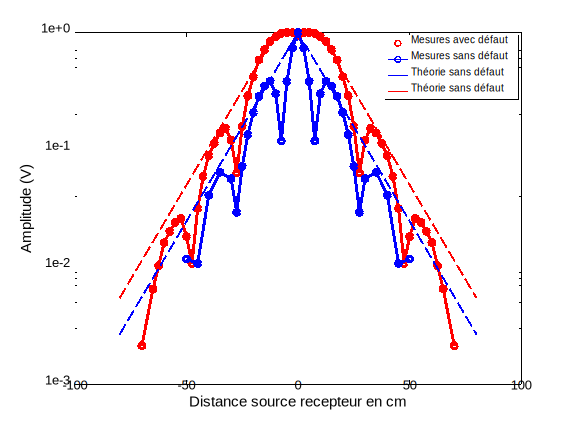
\includegraphics[width=0.5 \textwidth]{./images_chp3/comparaison_decroissance_log_theo.png}
\caption{\label{p_tube2} Amplitude du microphone mesurée dans le réseau avec un défaut à 2 résonateurs. À gauche en ordonnées linéaires, à droite en ordonnées logarithmiques, normalisée.}
\end{figure}

Dans le cas sans défaut, la décroissance mesurée est légèrement plus importante que celle simulée, en raison des pertes dues aux fuites.

Dans le cas avec défaut, la pression ne décroît pas dans la première cellule (sur les 10 premiers centimètres, correspondant à la distance source-défaut) car le défaut résonne. Il y a ensuite une décroissance équivalente à celle d'un réseau sans défaut.
Une onde de forte amplitude est donc bien localisée au niveau de la singularité. Mais le défaut ne semble pas agir sur le reste du réseau. \\~\\

\todo{2 réseaux, soit 2 k ? pb source ?}

\todo{normalisé} 

%Les décroissances sont les mêmes pour les 2 courbes : le défaut a donc juste pour effet d'augmenter le niveau sonore mais n'induit pas une décroissance plus forte.


